\subsection{Visualizing Stress On Hexahedron}
Moreover, as is mentioned before, the most significant benefit obtained from using equal-sized voxels is the potentail to simply construct
the element stiffness matrix $\bK^e$ once and even get rid of the global assembly procedure. To generate comparable visualizations effectively, our strategy is to first conservatively voxelize
the original tetdrahedron mesh, where each point (not just vertex) on the tetrahedron mesh is contained inside the voxelization, and then compute and map the nodal displacements on each grid points back to the input mesh in terms of trilinear interpolation.
Here we experimented with voxelizations under different resolutions with $k = 8, 18, 28, 38, 58$, where $k$ denotes the number of voxels of the bounding box along $x$ direction.

\begin{figure}[!htbp]
    \begin{center}
        $k=8$
        \quad
        \begin{subfigure}[b]{0.4\textwidth}
            \centering
            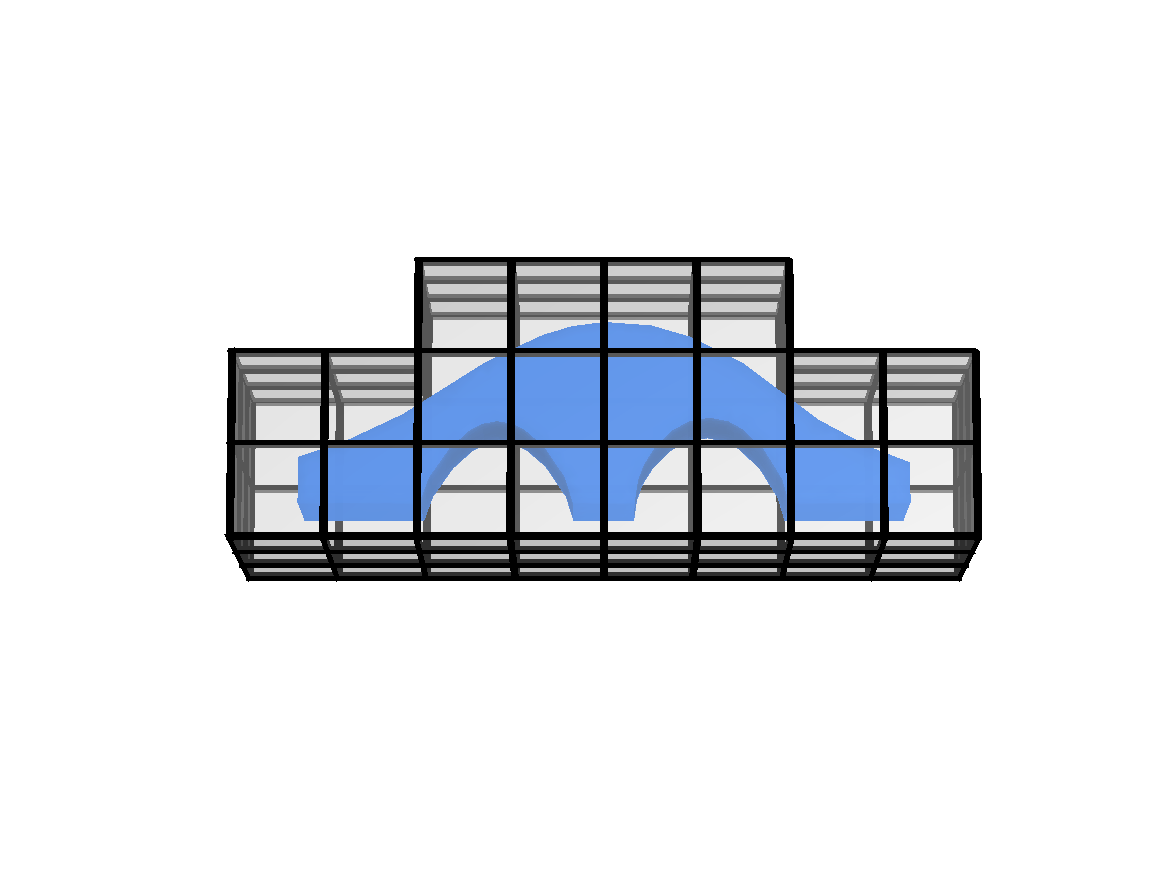
\includegraphics[width=\textwidth]{hex/resized/archbridge_cage_1}
        \end{subfigure}
        \begin{subfigure}[b]{0.35\textwidth}
            \centering
            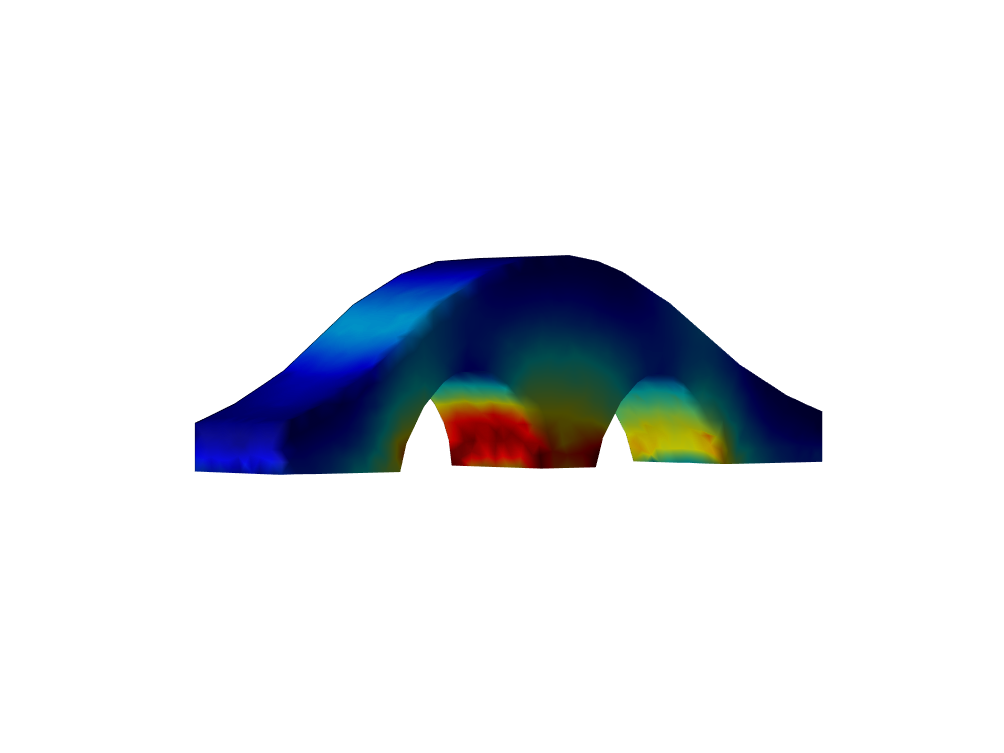
\includegraphics[width=\textwidth]{hex/resized/archbridge_1}
        \end{subfigure}\\ 

        $k=18$
        \quad
        \begin{subfigure}[b]{0.4\textwidth}
            \centering
            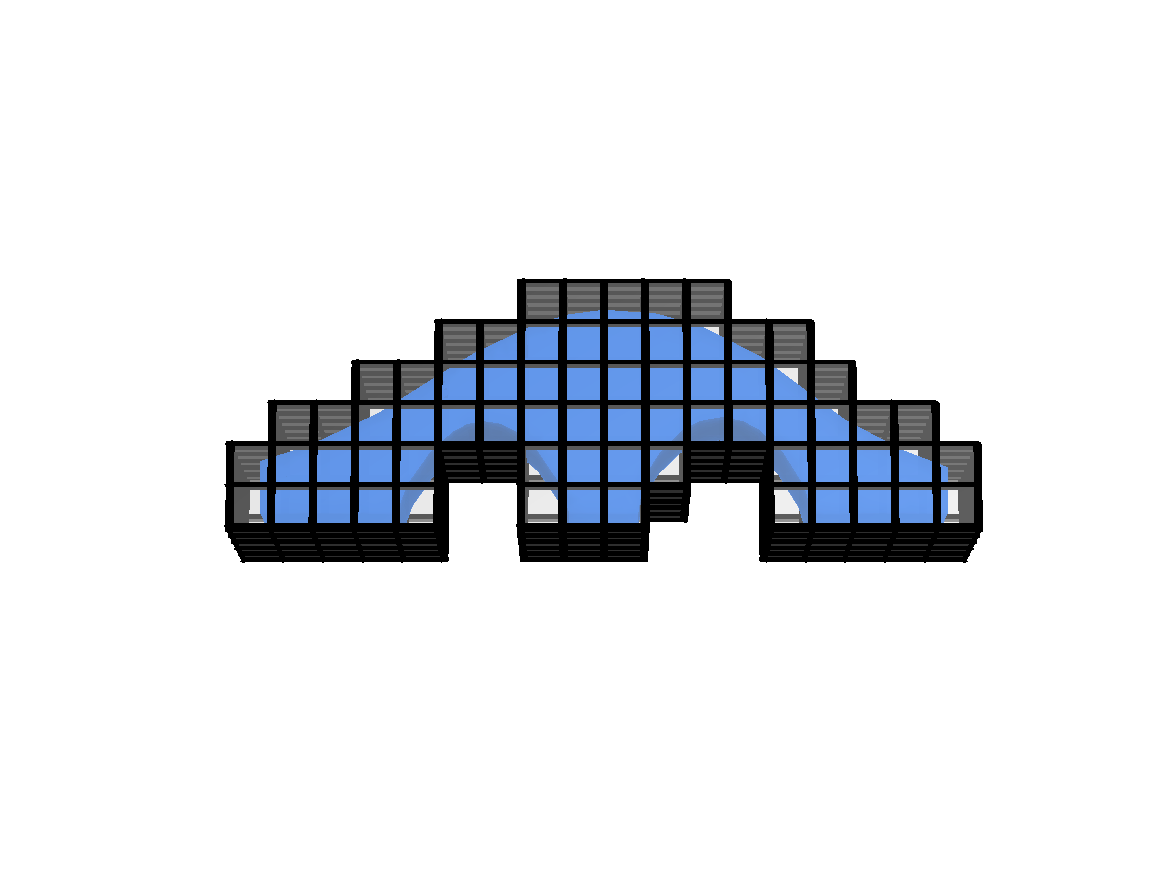
\includegraphics[width=\textwidth]{hex/resized/archbridge_cage_2}
        \end{subfigure}
        \begin{subfigure}[b]{0.35\textwidth}
            \centering
            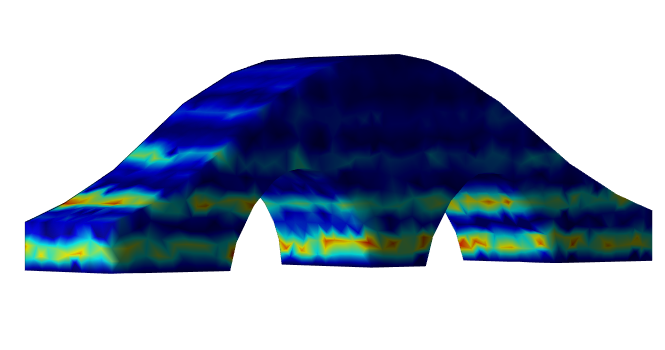
\includegraphics[width=\textwidth]{hex/resized/archbridge_2}
        \end{subfigure}\\ 


        $k=28$
        \quad
        \begin{subfigure}[b]{0.4\textwidth}
            \centering
            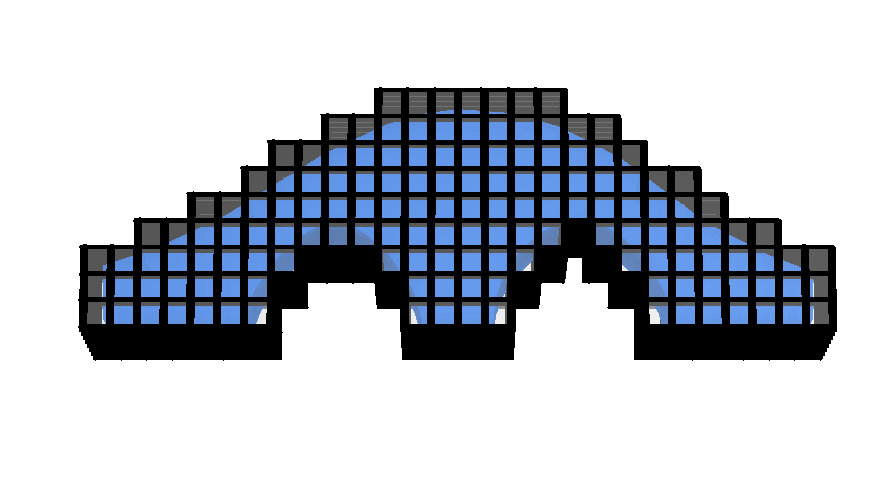
\includegraphics[width=\textwidth]{hex/resized/archbridge_cage_3}
        \end{subfigure}
        \begin{subfigure}[b]{0.35\textwidth}
            \centering
            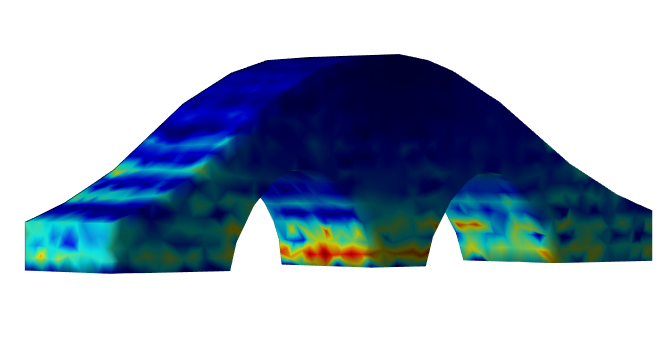
\includegraphics[width=\textwidth]{hex/resized/archbridge_3}
        \end{subfigure}\\ 


        $k=38$
        \quad
        \begin{subfigure}[b]{0.4\textwidth}
            \centering
            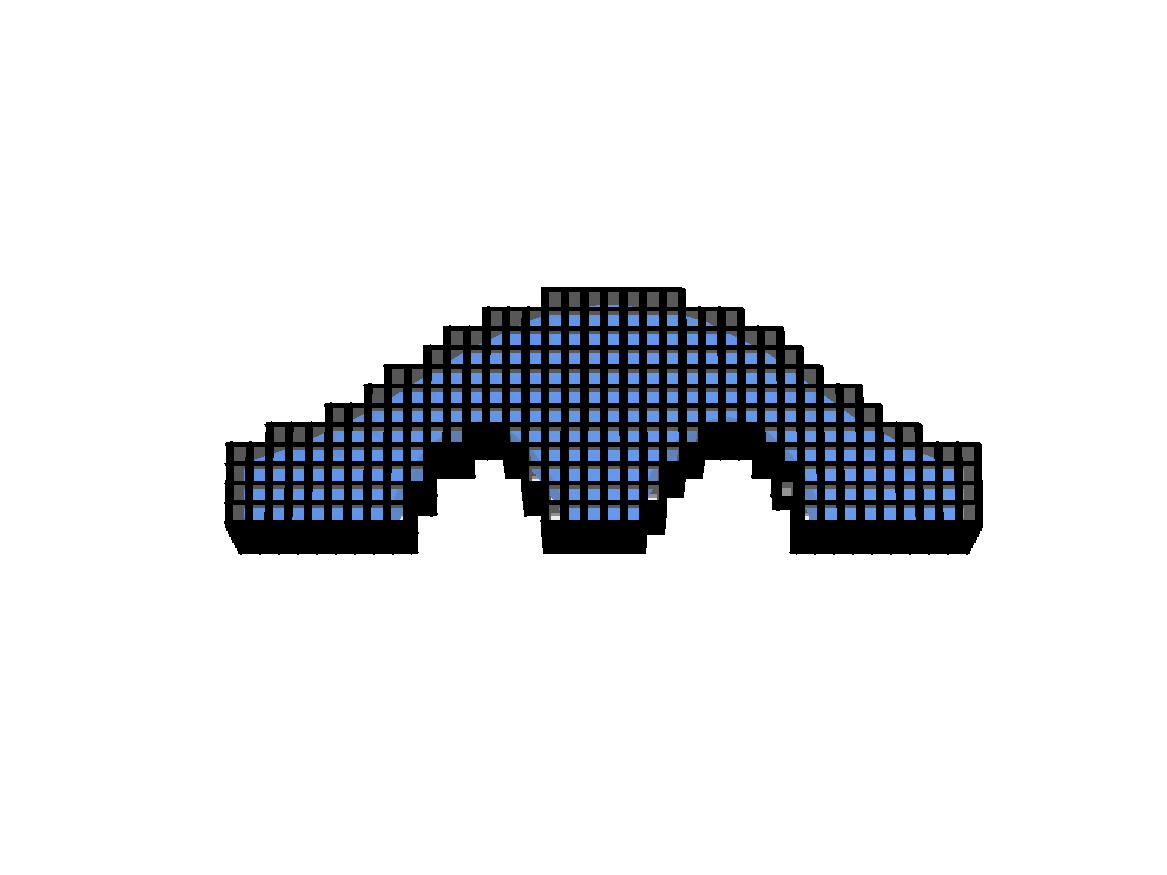
\includegraphics[width=\textwidth]{hex/resized/archbridge_cage_4}
        \end{subfigure}
        \begin{subfigure}[b]{0.35\textwidth}
            \centering
            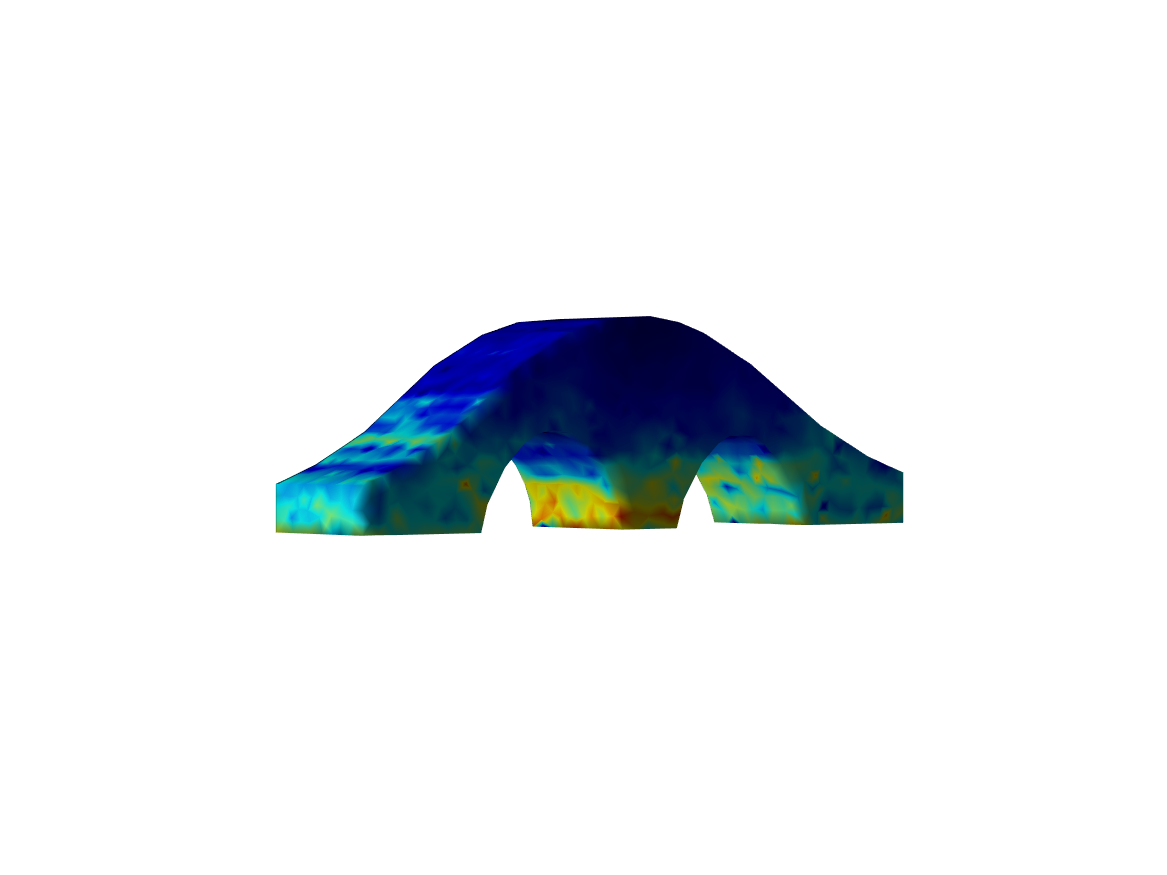
\includegraphics[width=\textwidth]{hex/resized/archbridge_4}
        \end{subfigure}\\ 


        $k=58$
        \quad
        \begin{subfigure}[b]{0.4\textwidth}
            \centering
            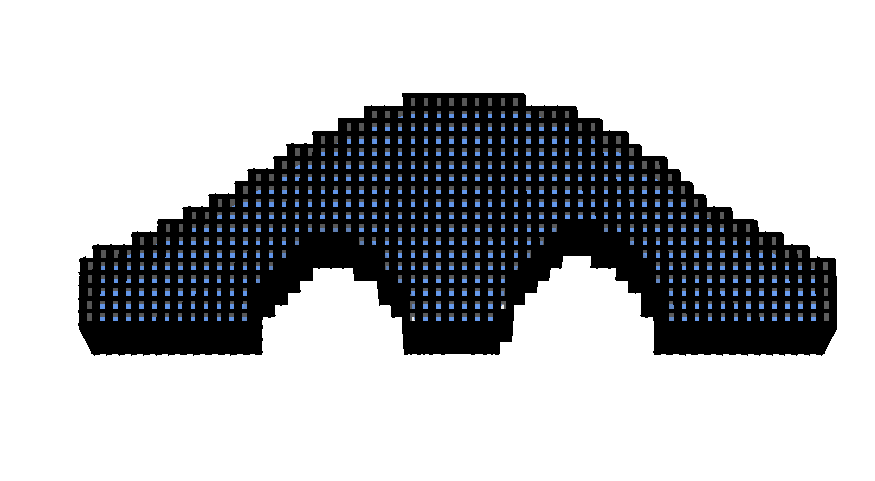
\includegraphics[width=\textwidth]{hex/resized/archbridge_cage_5}
        \end{subfigure}
        \begin{subfigure}[b]{0.35\textwidth}
            \centering
            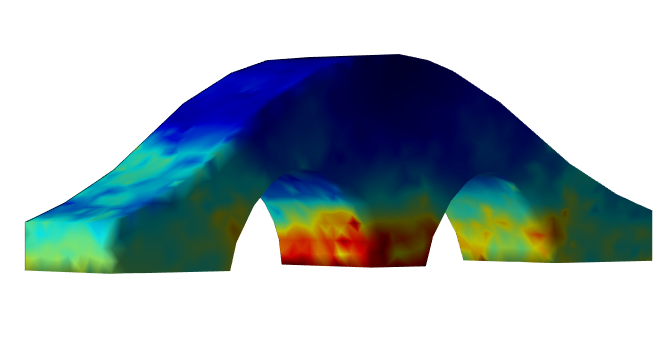
\includegraphics[width=\textwidth]{hex/resized/archbridge_5}
        \end{subfigure}\\ 


        \caption{\label{fig:5} von Mises' effective stress field generated from interpolated hexahedral nodal displacements}
    \end{center}
\end{figure}